\section{PTracking Algorithm}

\begin{frame}
	\frametitle{PTracking}
	\framesubtitle{Distributed Particle Filtering for Multi-Sensor Multiple Object Tracking}
	
	\LARGE
	
	\begin{block}{Idea}
		Achieving \textbf{high} precision and robustness, as a global method does, while trying to keep
		a \textbf{low} computational load in order to obtain \textbf{real-time} performance, as
		recursive methods do
	\end{block}
\end{frame}

\begin{frame}
	\frametitle{PTracking}
	\framesubtitle{Contributions}
	
	\Large
	
	\vspace{0.2cm}
	
	We propose a novel technique based on \emph{Distributed Particle Filtering}. The key contributions
	are:
	
	\vspace{0.15cm}
	
	\begin{enumerate}
		\item \textbf{Real-time} multiple object tracking method
		\item Novel clustering method that \textbf{keeps} track of multiple objects whose number is
			  \textbf{not known} a priori, ensuring a \textbf{limited} Gaussian distribution in the
			  particle space
		\item \textbf{Asynchronous} algorithm to improve robustness with respect to communication
			  failures and dead nodes
	\end{enumerate}
\end{frame}

\begin{frame}
	\frametitle{PTracking}
	\framesubtitle{General Schema}
	
	\vspace{-0.27cm}
	
	\begin{columns}[T]
		\column{.5\textwidth}
		
		\vspace{0.8cm}
		
		\begin{itemize}
			\item \textbf{Input:} set of positions of the objects provided by a multi object detector
				  system (e.g., \cite{Bloisi12})
			
			\vspace{1.6cm}
			
			\item \textbf{Output:} set of estimated trajectories of the moving objects over time
		\end{itemize}
		
		\column{.5\textwidth}
		\centering
		
		\begin{tikzpicture}
			\node at (0,0) [draw=black,ultra thick,inner sep=0pt]
			{
				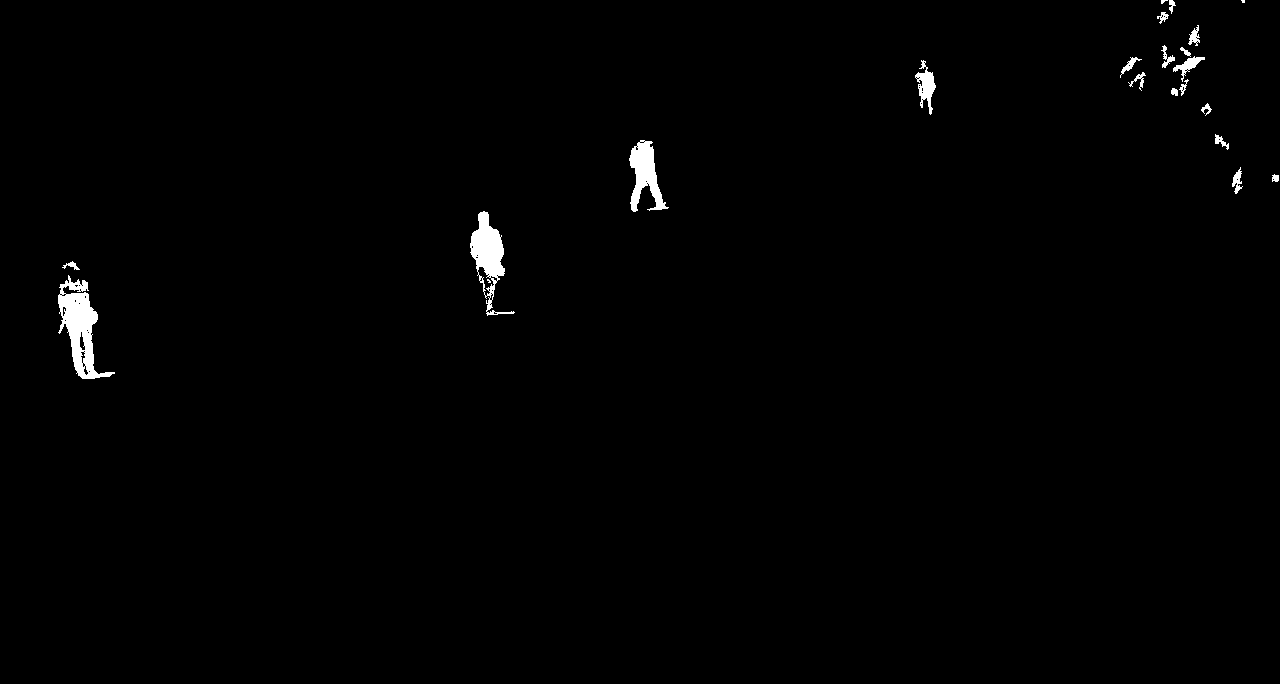
\includegraphics[width=6cm]{Figures/Detection}
			};
			\node at (0,-3.35) [draw=black,ultra thick,inner sep=0pt]
			{
				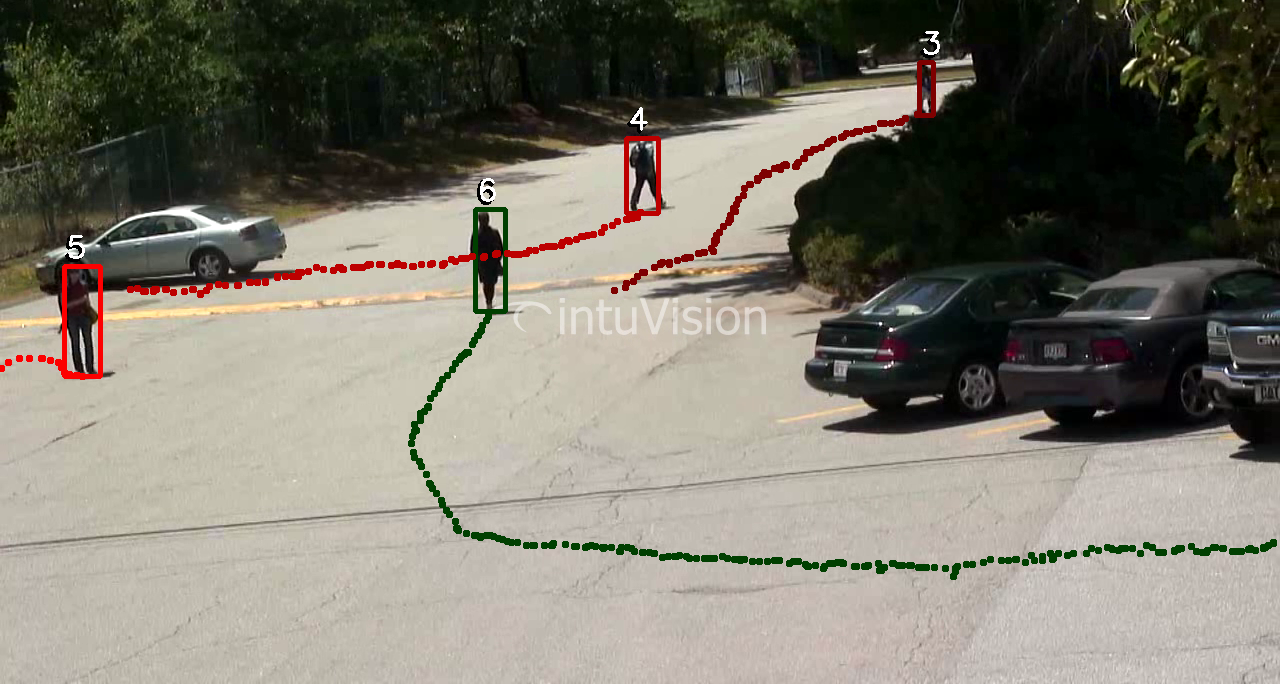
\includegraphics[width=6cm]{Figures/Tracking}
			};
		\end{tikzpicture}
	\end{columns}
	
	\vspace{0.3cm}
	
	\tiny
	
	\cite{Bloisi12} D. D. Bloisi \emph{et al.},  ``Independent Multimodal Background Subtraction'',
	CompIMAGE, 2012
\end{frame}

\begin{frame}
	\frametitle{PTracking}
	\framesubtitle{Pseudo-code}
	
	\begin{columns}[T]
		\column{.05\textwidth}
		
		\column{.55\textwidth}
		
		\only<1>
		{
			\begin{algorithm}[H]
				\tiny
				\KwIn{perceptions $ z_{s,t} $, local track numbers $ oi_{s,t-1} $, global track numbers $ OI_{s,t-1} $}
				\BlankLine
				\KwData{set of local particles $ \tilde{\xi}_{s,t} $, set of global particles $ \tilde{\xi}_{\mathcal{S'},t} $, sensor pose $ m_{s,t} $, local GMM set $ \mathcal{L} $, global GMM set $ \mathcal{G} $}
				\BlankLine
				\KwOut{global estimations $ x_{s,t} = (\boldsymbol{OI}_{s,t},\boldsymbol\Lambda_{s,t},\boldsymbol{M}_{s,t},\boldsymbol\Sigma_{s,t}) $}
				\BlankLine
				\Begin
				{
					\textcolor{darkgreen}{$ \tilde{\xi}_{s,t} \sim \pi_t (x_{s,t} | x_{s,t-1},z_{s,t},m_{s,t}) $}
					\BlankLine
					\textcolor{darkgreen}{Re-sample by using the SIR principle}\\
					\BlankLine
					\textcolor{darkgreen}{$ \mathcal{L} = KClusterize(\tilde{\xi}_{s,t}) $}
					\BlankLine
					\textcolor{darkgreen}{$ (\boldsymbol{oi}_{s,t},\boldsymbol\lambda_{s,t},\boldsymbol\mu_{s,t},\boldsymbol\sigma_{s,t}) = DataAssociation(\mathcal{L}, oi_{s,t-1}) $}
					\BlankLine
					\textcolor{darkgreen}{Communicate belief $ (\boldsymbol{oi}_{s,t},\boldsymbol\lambda_{s,t},\boldsymbol\mu_{s,t},\boldsymbol\sigma_{s,t}) $ to other agents}
				}
				\BlankLine
				\Begin
				{
					Collect $ \mathcal{L}_{S'} $ from a subset $ \mathcal{S'} \subseteq \mathcal{S} $ of
					sensors within a $ \Delta t $
					\BlankLine
					$ \tilde{\xi}_{\mathcal{S'},t} \sim \tilde\pi = \sum_{s \in \mathcal{S'}} \boldsymbol\lambda_{s,t} \, \mathcal{N} (\boldsymbol\mu_{s,t},\boldsymbol\sigma_{s,t}) $
					\BlankLine
					Re-sample by using the SIR principle\\
					\BlankLine
					$ \mathcal{G} = KClusterize(\tilde\xi_{{\mathcal{S'},t}}) $
					\BlankLine
					$ (\boldsymbol{OI}_{s,t},\boldsymbol\Lambda_{s,t},\boldsymbol{M}_{s,t},\boldsymbol\Sigma_{s,t}) = DataAssociation(\mathcal{G},OI_{s,t-1}) $
				}
			\end{algorithm}
			
			\column{.01\textwidth}
			
			\Huge
			\vspace{2.15cm}
			
			\begin{center}
				\textcolor{blue}{$ \Rightarrow $}
			\end{center}
			
			\column{.44\textwidth}
			
			\centering
			
			\begin{tikzpicture}
				\node at (0,0) [draw=black,ultra thick,inner sep=0pt]
				{
					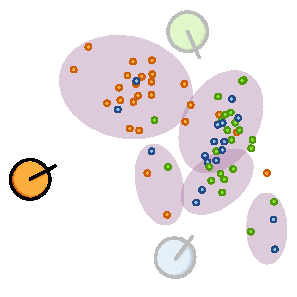
\includegraphics[width=3.3cm]{Figures/Mamot-1}
				};
				\node at (0,-3.5) [draw=black,ultra thick,inner sep=0pt]
				{
					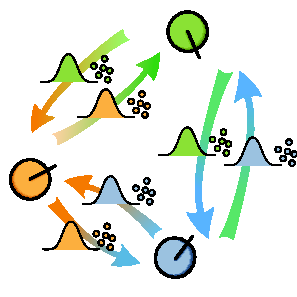
\includegraphics[width=3.3cm]{Figures/Mamot-2}
				};
			\end{tikzpicture}
		}
		
		\only<2->
		{
			\begin{algorithm}[H]
				\tiny
				\KwIn{perceptions $ z_{s,t} $, local track numbers $ oi_{s,t-1} $, global track numbers $ OI_{s,t-1} $}
				\BlankLine
				\KwData{set of local particles $ \tilde{\xi}_{s,t} $, set of global particles $ \tilde{\xi}_{\mathcal{S'},t} $, sensor pose $ m_{s,t} $, local GMM set $ \mathcal{L} $, global GMM set $ \mathcal{G} $}
				\BlankLine
				\KwOut{global estimations $ x_{s,t} = (\boldsymbol{OI}_{s,t},\boldsymbol\Lambda_{s,t},\boldsymbol{M}_{s,t},\boldsymbol\Sigma_{s,t}) $}
				\BlankLine
				\Begin
				{
					$ \tilde{\xi}_{s,t} \sim \pi_t (x_{s,t} | x_{s,t-1},z_{s,t},m_{s,t}) $
					\BlankLine
					Re-sample by using the SIR principle\\
					\BlankLine
					$ \mathcal{L} = KClusterize(\tilde{\xi}_{s,t}) $
					\BlankLine
					$ (\boldsymbol{oi}_{s,t},\boldsymbol\lambda_{s,t},\boldsymbol\mu_{s,t},\boldsymbol\sigma_{s,t}) = DataAssociation(\mathcal{L}, oi_{s,t-1}) $
					\BlankLine
					Communicate belief $ (\boldsymbol{oi}_{s,t},\boldsymbol\lambda_{s,t},\boldsymbol\mu_{s,t},\boldsymbol\sigma_{s,t}) $ to other agents
				}
				\BlankLine
				\Begin
				{
					\textcolor{lightred}{Collect $ \mathcal{L}_{S'} $ from a subset $ \mathcal{S'} \subseteq \mathcal{S} $ of sensors within a $ \Delta t $}
					\BlankLine
					\textcolor{lightred}{$ \tilde{\xi}_{\mathcal{S'},t} \sim \tilde\pi = \sum_{s \in \mathcal{S'}} \boldsymbol\lambda_{s,t} \, \mathcal{N} (\boldsymbol\mu_{s,t},\boldsymbol\sigma_{s,t}) $}
					\BlankLine
					\textcolor{lightred}{Re-sample by using the SIR principle}\\
					\BlankLine
					\textcolor{lightred}{$ \mathcal{G} = KClusterize(\tilde\xi_{{\mathcal{S'},t}}) $}
					\BlankLine
					\textcolor{lightred}{$ (\boldsymbol{OI}_{s,t},\boldsymbol\Lambda_{s,t},\boldsymbol{M}_{s,t},\boldsymbol\Sigma_{s,t}) = DataAssociation(\mathcal{G},OI_{s,t-1}) $}
				}
			\end{algorithm}
			
			\column{.01\textwidth}
			
			\Huge
			\vspace{2.15cm}
			
			\begin{center}
				\textcolor{blue}{$ \Rightarrow $}
			\end{center}
			
			\column{.44\textwidth}
			
			\centering
			
			\begin{tikzpicture}
				\node at (0,0) [draw=black,ultra thick,inner sep=0pt]
				{
					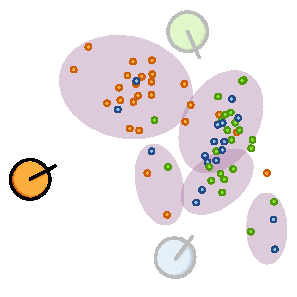
\includegraphics[width=3.3cm]{Figures/Mamot-1}
				};
				\node at (0,-3.5) [draw=black,ultra thick,inner sep=0pt]
				{
					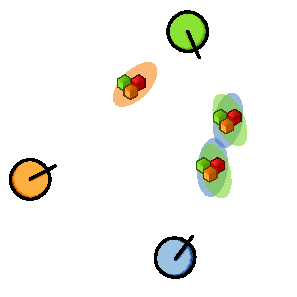
\includegraphics[width=3.3cm]{Figures/Mamot-3}
				};
			\end{tikzpicture}
		}
	\end{columns}
\end{frame}

\begin{frame}
	\frametitle{PTracking}
	\framesubtitle{Group Tracking}
	
	\begin{figure}
		\begin{tikzpicture}[map/.style={draw=black,ultra thick,inner sep=0pt}]
			\node at (0,0) [map] {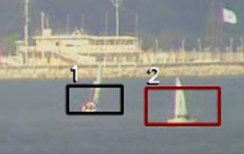
\includegraphics[width=0.32\linewidth]{Figures/GroupTracking-a}};
			\node at (4,0) [map] {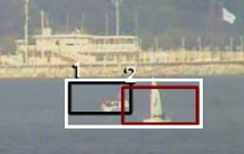
\includegraphics[width=0.32\linewidth]{Figures/GroupTracking-b}};
			\node at (8,0) [map] {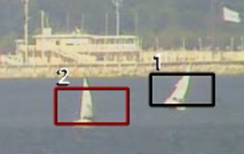
\includegraphics[width=0.32\linewidth]{Figures/GroupTracking-c}};
		\end{tikzpicture}
		\caption{Group tracking. Two sailing boats are going to cross each other. Occlusions are handled
				 considering the collapsing tracks to form a group, instead of tracking them
				 separately.}
	\end{figure}
\end{frame}

\begin{frame}
	\frametitle{KClusterize}
	\framesubtitle{Contributions}
	
	\Large
	
	\emph{KClusterize} has been designed aiming at fulfilling the following three requirements:
	
	\begin{enumerate}
		\item \textbf{Number} of objects to be detected \textbf{cannot} be known a priori
		\item \textbf{Low} computational load for real-time applications
		\item \textbf{Gaussian distribution} for each cluster
	\end{enumerate}
\end{frame}

\begin{frame}
	\frametitle{KClusterize}
	\framesubtitle{Typical Clustering Scenario}
	
	\vspace{0.5cm}
	
	\begin{figure}[!t]
		\begin{minipage}[l]{0.23\textwidth}
			\vspace*{\fill}
			\centering
			\subfigure[Analysed situation.]
			{
				\begin{tikzpicture}[map/.style={draw=white,ultra thick,inner sep=0pt}]
					\node at (0,0) [map]
					{
						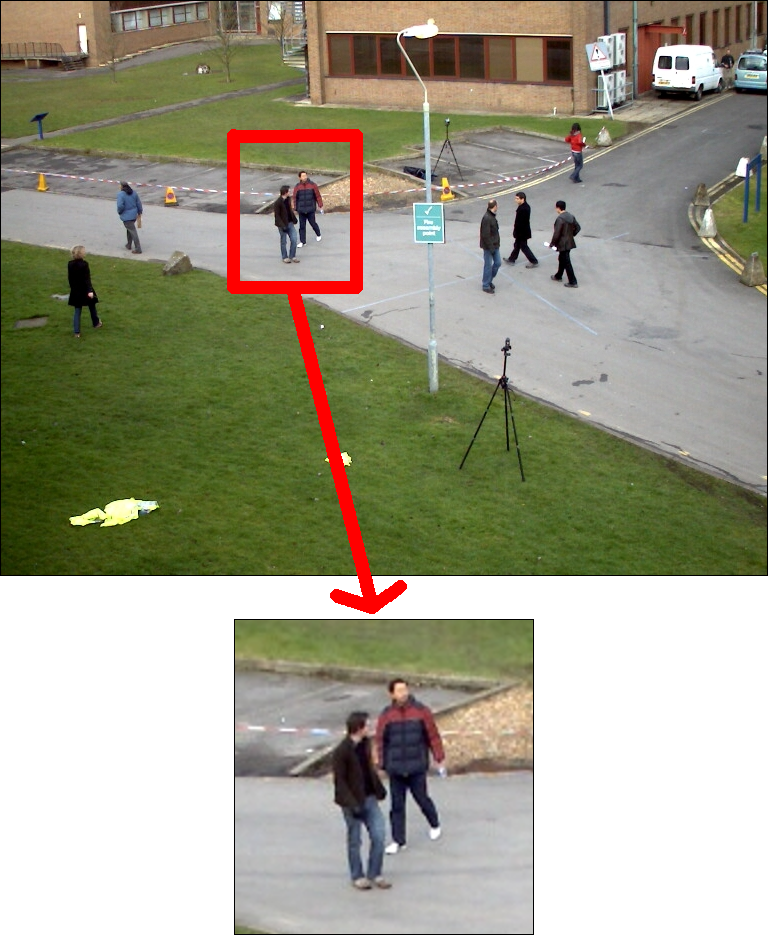
\includegraphics[width=\linewidth]{Figures/PETS-2009-Frame-0722-zoomed}
					};
				\end{tikzpicture}
			}
		\end{minipage}
		\hspace{0.1cm}
		\begin{minipage}[c]{0.74\textwidth}
			\subfigure[K-means with $ k = 2 $.]
			{
				\begin{tikzpicture}[map/.style={draw=white,ultra thick,inner sep=0pt}]
					\node at (0,0) [map]
					{
						\includegraphics[width=0.47\linewidth]{Figures/Kmeans-2.png}
					};
				\end{tikzpicture}
			}
			\hspace{-3.8mm}
			\subfigure[Hierarchical Clustering.]
			{
				\begin{tikzpicture}[map/.style={draw=white,ultra thick,inner sep=0pt}]
					\node at (0,0) [map]
					{
						\includegraphics[width=0.47\linewidth]{Figures/HierarchicalClustering.png}
					};
				\end{tikzpicture}
			}
			
			\subfigure[QT-Clustering.]
			{
				\begin{tikzpicture}[map/.style={draw=white,ultra thick,inner sep=0pt}]
					\node at (0,0) [map]
					{
						\includegraphics[width=0.47\linewidth]{Figures/QT-Clustering.png}
					};
				\end{tikzpicture}
			}
			\hspace{-3.8mm}
			\subfigure[KClusterize.]
			{
				\begin{tikzpicture}[map/.style={draw=white,ultra thick,inner sep=0pt}]
					\node at (0,0) [map]
					{
						\includegraphics[width=0.47\linewidth]{Figures/KClusterize.png}
					};
				\end{tikzpicture}
			}
		\end{minipage}
	\end{figure}
\end{frame}

\begin{frame}
	\frametitle{KClusterize}
	\framesubtitle{Clustering Speed}
	
	\begin{figure}[t]
		\begin{tikzpicture}[map/.style={draw=white,ultra thick,inner sep=0pt}]
			\node at (0,0) [map]
			{
				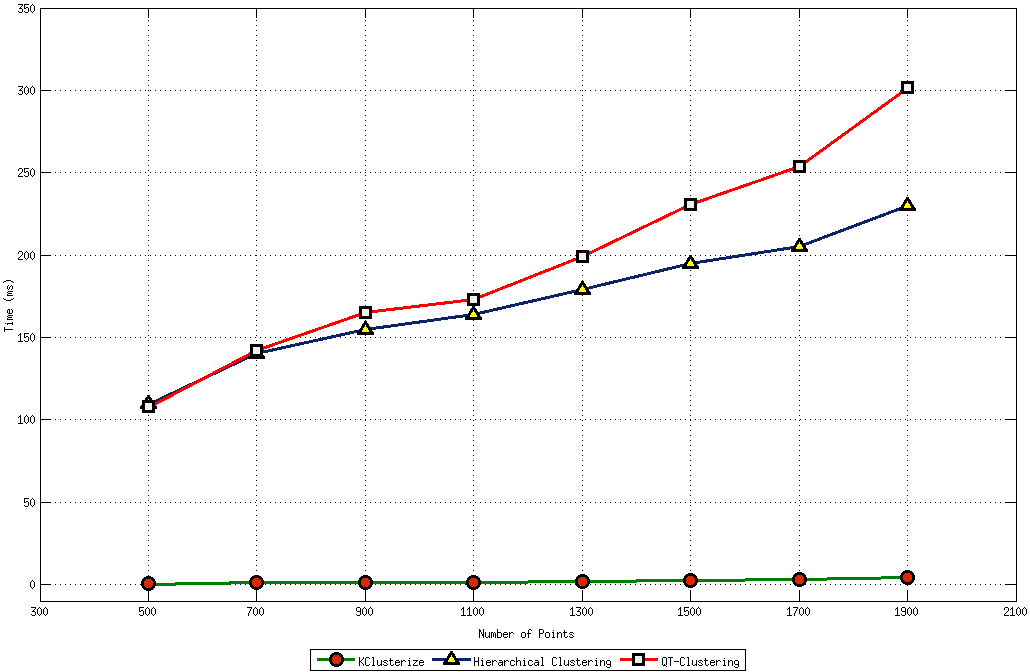
\includegraphics[width=0.88\linewidth]{Figures/ClusteringComparison}
			};
		\end{tikzpicture}
	\end{figure}
\end{frame}

\begin{frame}
	\frametitle{KClusterize}
	\framesubtitle{Cluster Gaussian Distribution}
	
	\vspace{0.3cm}
	
	\setcounter{subfigure}{0}
	
	\begin{figure}[!t]
		\centering
		\subfigure[Output of the algorithm on frame \#269.]
		{
			\begin{tikzpicture}[map/.style={draw=black,ultra thick,inner sep=0pt}]
				\node at (0,0) [map]
				{
					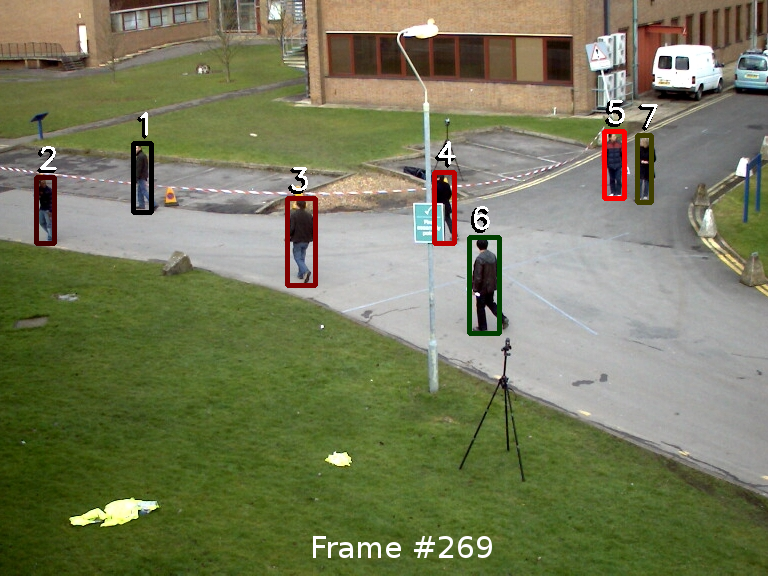
\includegraphics[width=0.48\linewidth]{Figures/KClusterize-Frame-0269-Output.png}
				};
			\end{tikzpicture}
		}
		\hspace{-3.8mm}
		\subfigure[A 2D visualization of frame \#269.]
		{
			\begin{tikzpicture}[map/.style={draw=white,ultra thick,inner sep=0pt}]
				\node at (0,0) [map]
				{
					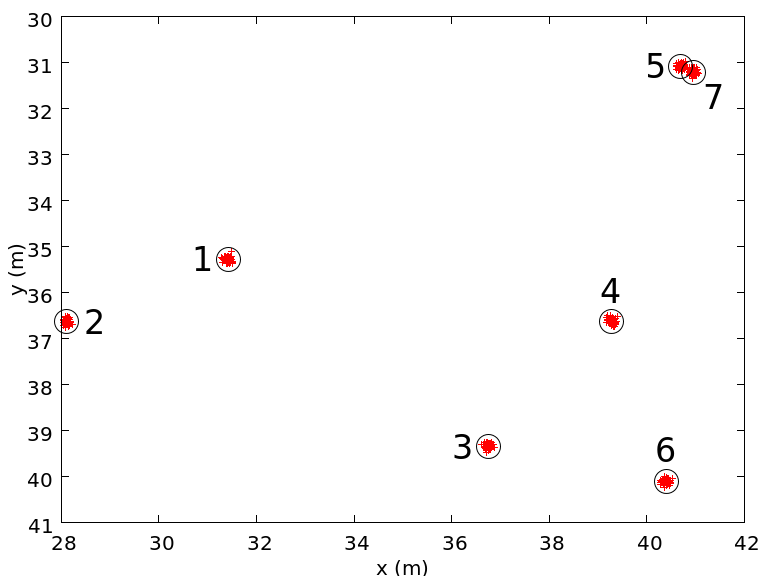
\includegraphics[width=0.48\linewidth]{Figures/KClusterize-Frame-0269-PlaneView.png}
				};
			\end{tikzpicture}
		}
	\end{figure}
\end{frame}
